\hthree{Die "App"-Klasse}\label{sec:app}

Die "App"-Klasse ist die Klasse, welche die alle Endpunkte verwaltet.  

\begin{figure}[H]
    \centering
    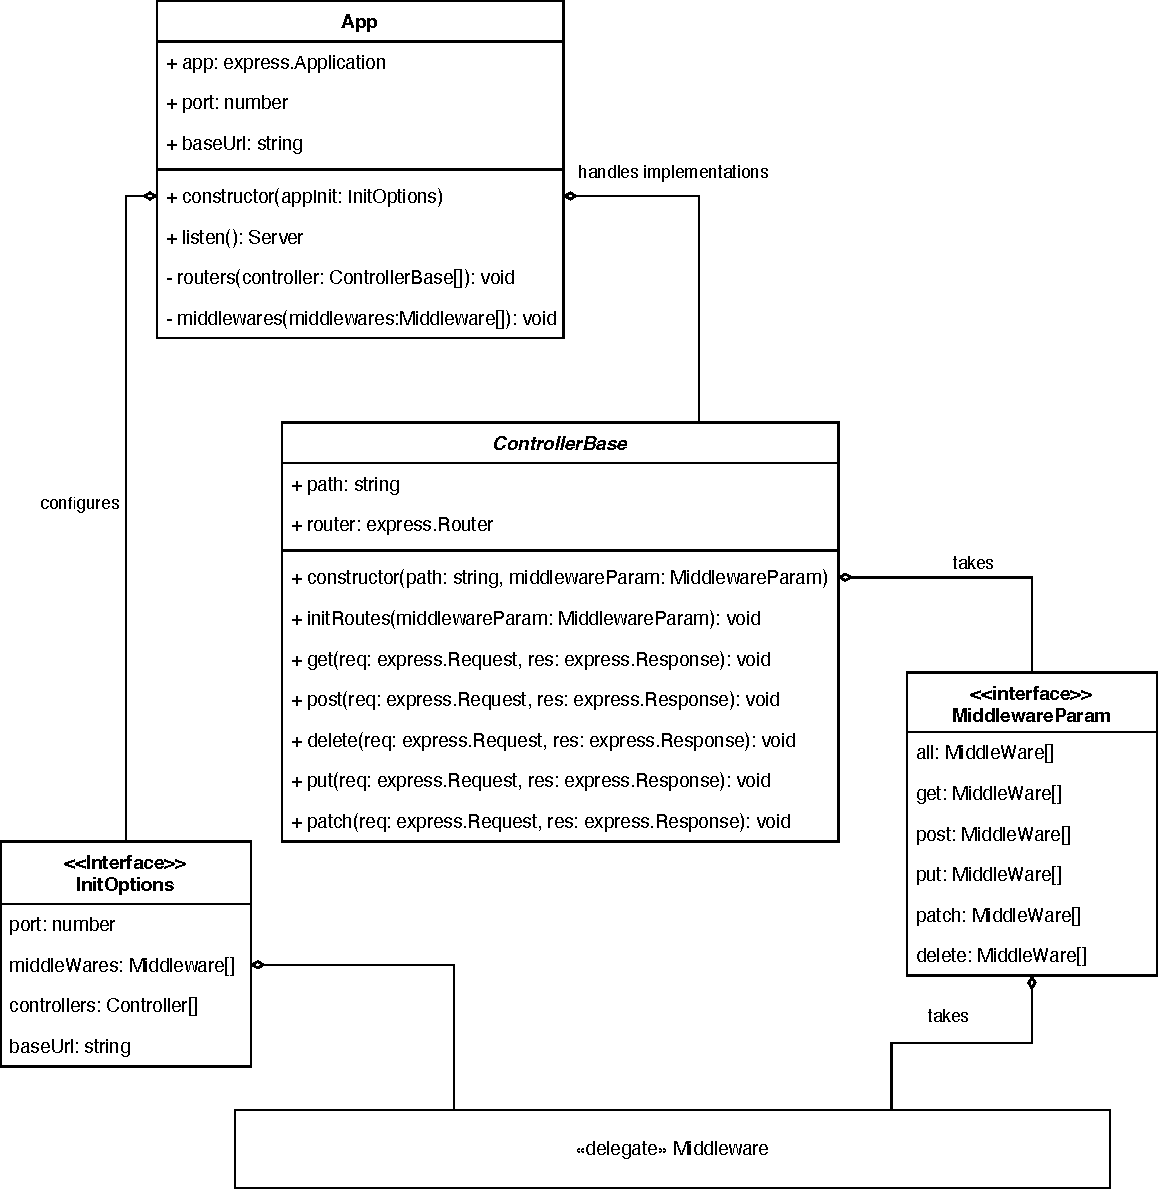
\includegraphics[width=\textwidth]{media/APITemplate/apiArchitecture.svg.pdf}
    \caption{UML Diagramm der API-Architektur}
    \label{fig:apiUML}
\end{figure}

Im Konstruktor der App-Klasse können verschiedene Optionen mitgegeben werden:

\hfive{"Port"}

Durch die Port-Option kann angegeben werden, auf welchem Port die API HTTP-Requests annehmen soll. Standardmäßig ist dies auf die Umgebungsvariable "PORT" gesetzt. Falls diese nicht gesetzt ist, wird der Port 3001 verwendet.

\hfive{"Controllers"}

Die Controller werden als Array von Controller Objekten übergeben und repräsentieren einen Endpoint. Siehe Unterpunkt \ref{sec:controller} Controller

\hfive{"Middlewares"}

Dies ist ein Array an Middlewares, welche bei jedem Request ausgeführt werden. Siehe Unterpunkt \ref{sec:middleware} Middleware

\hfive{"Base-URL"}

Durch diesen String kann der Root-Pfad definiert werden. Standardmäßig ist diese auf "/" gesetzt. Bei Zelia ist diese auf "/api" konfiguriert worden, da alle API bezogenen Anfragen auf den Pfad "/api" gehen.

Die "listen"-Methode muss aufgerufen werden, um die "App" zu starten.
Verwendung der "App"
Um eine Instanz der App-Klasse zu erstellen, muss diese importiert werden. Danach kann die "App" mit ihren registrierten "Controllern" und "Middlewares" instanziiert werden. Damit die "App” auf dem angegebenen Port gestartet wird, wir die listen Methode aufgerufen.

\typescript{code/APITemplate/appusage.ts}{Verwendung der App-Klasse}